\documentclass{llncs}
\usepackage{makeidx}  
\usepackage{ifthen}
\usepackage{amssymb}
\usepackage{graphicx}

\newboolean{showcomments}
\setboolean{showcomments}{false}
\ifthenelse{\boolean{showcomments}}
  {\newcommand{\bnote}[2]{
	\fbox{\bfseries\sffamily\scriptsize#1}
    {\sf\small$\blacktriangleright$\textit{#2}$\blacktriangleleft$}
   }
  }
  {\newcommand{\bnote}[2]{}
  } 


% Package for including code in the document
\usepackage{listings}
\lstdefinelanguage{javascript}{
   morekeywords={break,do,instanceof,typeof,case,else,new,var,catch,finally,return, void, continue, for, switch, while, debugger, function, this, with, default, if, throw, delete, in, try, class, enum, extends, super, const, export, import, implements, let, private, public, interface, package,protected, static, yield},
   keywordstyle=\ttfamily\bfseries,
   basicstyle=\ttfamily\small,
   ndkeywords={},
%                >>>=
%              , >>= , >>> , === , !==, <<=
%              , +=  , -=  , *=  , %= , >=
%              , ==  , !=  , ++  , -- , <<
%              , >>  , <=  , &=  , ,= , ^=
%              , &&  ,
%              , {     , }     , (     , )    , [   , ]
%              , .     , ;     , ,     , <    , >   , !
%              , ~     , =     , &     , ,    , ^   , ?
%              , :     , *     , %     , +    , -
   ndkeywordstyle=\ttfamily\bfseries,
   identifierstyle=\ttfamily,
   sensitive=false,
   comment=[l]{//},
   morecomment=[s]{/*}{*/}, 
   commentstyle=\rmfamily,
   stringstyle=\ttfamily,
   columns=flexible,
   showstringspaces=false,
   numbers=left,
   numberstyle=\tiny,
   stepnumber=1,
   numbersep=5pt,
   numberblanklines=false
}

% suppress counting of empty lines in lstlistings, thanks to: http://tex.stackexchange.com/questions/33999/suppress-line-numbering-for-empty-lines-in-listings-package
\makeatletter
\lst@AddToHook{OnEmptyLine}{\addtocounter{lstnumber}{-1}}% Remove line number increment from listings
\makeatother

\usepackage{hyperref}
\newcommand{\myurl}[1]{{\href{http://#1}{\texttt{#1}}}}
\newcommand{\myurlt}[2]{{\href{http://#1~#2}{\tt #1{\twiddle}#2}}}
\newcommand{\myurlh}[3]{{\href{http://#1#3}{\tt #1#2#3}}}



\begin{document}
\sloppypar


\title{Distributed Electronic Rights in JavaScript}

\author{Mark S. Miller\inst{1} \and Tom Van Cutsem\inst{2} \and Bill Tulloh\inst{3} }

\institute{Google, Inc. \and Vrije Universiteit Brussel \and George Mason University}

\maketitle    

\begin{abstract}

Smart Contracts are cool. \bnote{Mark}{need a real abstract}
\bnote{Mark}{Explain that it is a Progress Report here rather than in title.}

\keywords{security, distributed objects, capabilities, smart contracts}
\end{abstract}

\section{Smart Contracts for the Rest of Us}

The fabric of the global economy is held together by contracts. A contract is an agreed arrangement for cooperation between mutually suspicious parties. But existing contracts are ambiguous, jurisdictions-specific, and written, interpreted, and adjudicated only by expensive experts. \emph{Smart contracts} are contract-like arrangements expressed in program code, where the behavior of the program enforces the terms of the ``contract''\cite{szabo1997formalizing}. Though not a substitute for legal contracts, they can provide some of the benefits of contracts for fine-grain, jurisdiction-free, and automated arrangements for which legal contracts are impractical.\footnote{
%
Although \emph{types as contracts}~\cite{DBLP:journals/computer/Meyer92} and \emph{higher order contracts}~\cite{findler2002contracts} can be seen as very special cases of smart contracts, their purpose is typically different: locating bugs during development rather than protection from misbehavior in the wild.}

To realize this potential, smart contracts themselves need a distributed, secure, persistent, and ubiquitous computational fabric. To avoid merely substituting one set of expensive experts for another, non-experts should be able to write smart contracts understandable by other non-experts.

We are working towards turning JavaScript into such a fabric. JavaScript is already understood and used by many non-expert programmers. We call our target JavaScript platform \emph{Dr. SES} for \emph{Distributed Resilient Secure EcmaScript}.\footnote{
%
The official standards name for JavaScript is ``EcmaScript''.
%
} We explain how it relates to today's JavaScript, and report on our progress building Dr. SES. To demonstrate that Dr. SES would be a suitable platform, we present a representative simple smart contract, \emph{secure distributed escrow exchange}, implemented in only 42 lines of JavaScript code. We also present a generic contract host, able to host this contract and others, in only 36 lines.

\section{Dr. SES: Distributed Resilient Secure EcmaScript}

Dr. SES is a platform for distributed, resilient and secure computing, layered on EcmaScript. How do these ingredients support electronic rights and contracts?

Dr. SES is layered on top of EcmaScript for two primary reasons. First is the ubiquity of the language. Due to its embedding in the browser, EcmaScript is available on a wide range of platforms. Second, because of this ubiquity, JavaScript is widely adopted among programmers.

In an architecture that aims to express electronic rights or contracts, security must play a key role. Dr. SES builds upon the object-capability paradigm. Capability principles are followed both to secure distributed objects as well as to secure the local execution environment. The latter allows Dr. SES programs to execute mobile code from untrusted parties without fear of granting excess privileges to that piece of code. This is especially relevant in the context of JavaScript, where mobile code is routinely sent from servers to clients. In Section~\ref{sec:contract_host}, we will show an example that  depends on the ability to safely execute third-party code.

JavaScript is not a distributed programming language. In the browser, a large number of APIs is available to scripts to communicate with servers and other frames, but these APIs are tedious to work with, and not designed with least-authority rules. That is why Dr. SES extends the JavaScript language proper with a handful of features to support least-authority distributed programming at the level of individual objects.

Finally, the resilience aspect of Dr. SES deals with the unavoidable issues of failure handling that come up in distributed systems.
%It is widely appreciated that writing correct, bug-free code in the presence of arbitrary failures is hard. Dr. SES, then, tries to make it as easy as possible for non-experts to deal with distributed failures.
Server-side Dr. SES programs periodically checkpoint their entire state, so that in the event of a failure, the program can always recover to a previously consistent state. Such Dr. SES programs can survive failures without any effort on the part of the programmer.

%Objects and object references in Dr. SES are always persistent, meaning that they survive arbitrary failures by default.

The current JavaScript standard, EcmaScript 5 (ES5), enables the \emph{SES} library to efficiently enforce local object-capability security rules on newly loaded JavaScript code. The \emph{Q} library turns JavaScript into a securable distributed object system, spanning both browsers and servers. The \emph{NodeKen} project is layering the Node server-side JavaScript implementation onto the Ken system~\cite{Yoo:CKen} for distributed orthogonal persistence---resilient against many failures. We explain each below.

Dr. SES is not specifically tied to electronic rights or contracts per se. Its focus is to make distributed programming in JavaScript as effortless as possible. Given such a platform, it then becomes possible to implement contracts with very little code. This is precisely what we will demonstrate in the second part of this paper, after having explained Dr. SES in more detail.



\subsection{Just Enough JavaScript}

JavaScript is a complex language, but this paper depends only on a small subset with two core constructs, \emph{functions} and \emph{records}. 

For the sake of brevity, this paper borrows one syntactic convenience proposed for ES6, \emph{arrow functions}~(``{\tt =>}''), and one proposed for ES7, the \emph{eventual-send operator}~(``{\tt !}''). Expanding away these conveniences, all the code here is working ES5 code, and is available at \myurl{code.google.com/p/es-lab/source/browse/trunk/src/ses/\#ses} and its {\tt contract} subdirectory.

\paragraph{Arrow functions.} 

The following five lines all define a one parameter function which returns twice its parameter. All bind a local variable named ``{\tt double}'' to this function. The first two lines are of historic interest only. This paper uses only the arrow function syntax of the last three lines.

\begin{verbatim}
  function double(n) { return n+n; }        // old function decl
  var double = function(n) { return n+n; }; // old function expr
  var double = (n) => { return n+n; };      // ES6 arrow function
  var double = (n) => n+n;    // non-"{" expr implicitly returned
  var double = n => n+n;      // parens optional if one param
\end{verbatim}

\paragraph{Records.} 

The record syntax {\tt \{x: 3, y: 4\}} is an expression that evaluates to a record with two named properties initialized to the values shown. Records and functions compose together naturally to give objects:

\begin{verbatim}
var makePoint = (x, y) => {
  return {
    getX: () => x,
    getY: () => y,
    add: other => makePoint(x + other.getX(), y + other.getY())
  };
};

var pt = makePoint(3, 5).add(makePoint(2, 7));
\end{verbatim}

A record of functions hiding variables serves as an object of methods ({\tt getX, getY, add}) hiding instance variables ({\tt x, y}). The {\tt makePoint} function serves as a class-like factory for making new point instances.


\subsection{SES: Securing JavaScript}





SES is an object-capability-secure subset of JavaScript. Historically, there have been two contrasting views on how to secure shared resources. In the ACL (access control list) approach, every time a resource is used, an access control check is performed, checking if the requestor holds the right to use the resource. In this paradigm, resources are often coarse-grained. In the capability-based approach, a capability represents the right to perform a set of operations on a specific, designated resource. The very fact that an operation was performed \emph{via} a capability is sufficient proof that the operation is authorized. In capability-based systems, both access rights and resources are mostly fine-grained.

Object-capability security marries the ideas of capability-based security with standard object-oriented programming. An object reference represents the right to invoke only the public interface of a specific object.

To secure a JavaScript application using object-capability principles, we require two properties. First, a script (program) must be born powerless, i.e. there must be no powerful globally accessible objects, such as an {\tt XMLHttpRequest} object that allows the script to communicate with the outside world. But if a script is born powerless, then how can it interact with the outside world at all? The answer is that the creator of the script may \emph{endow} the newborn script with references to some powerful objects at birth. This is how the script comes to obtain its first external object references.

Once a script obtains a reference to an external object, we must establish rules as to what the script can do with the object, and how the script can come to acquire further object references. The rules are familiar to any object-oriented programmer: an object reference should only grant the ability to invoke an object's public interface. The object's private state should be encapsulated. Thus, an object can only come to acquire new object references via argument and result passing.

JavaScript by itself is not an object-capability-secure language, because scripts are not born powerless (A JavaScript environment is full of globally mutable state) and because plain JavaScript objects are not encapsulated. From a security perspective, there were three problems with JavaScript's objects:

\begin{itemize}
\item Records were fully mutable, allowing one client of a point to, for example, replace its {\tt getX} method, violating the assumptions of other clients. ES5 provides a {\tt freeze} primitive, used by the SES library to define the {\tt def} function for making a tamper proof object graph.
\item ES3 had six violations of static scoping. Three are fixed unconditionally by ES5. In addition, ES5 provides a \emph{strict mode}, enabled by the {\tt "use strict";} directive shown below, which fixes the remaining three violations. (Throughout the rest of this paper, strict mode is assumed without further notation.)  
\item Even aside from these scoping violations, ES3 functions were not encapsulated. However, ES5 strict functions are fully encapsulated.
\end{itemize}

\begin{verbatim}
"use strict";
var makePoint = (x, y) => {
  return def({
    getX: () => x,
    getY: () => y,
    add: other => makePoint(x + other.getX(), y + other.getY())
  });
};
\end{verbatim}

A \emph{tamper-proof} record of \emph{encapsulated} functions hiding \emph{lexical} variables can be a \emph{defensively consistent} object~\cite{RobustComposition}. An object is defensively consistent when it can defend its own invariants and provide correct service to its well behaved clients, despite arbitrary or malicious misbehavior by its other clients. Our revised {\tt makePoint} above makes defensively consistent points.

\bnote{Mark}{Other SES elements:}
All effects only by using references.
No powerful references by default -- all implicitly shared objects are transitively immutable. 


\begin{description}
\item[{\tt def(obj)}] xx

\item[{\tt confine(src, env)}] xx

\item[{\tt Nat(allegedNumber)}] xx

\item[{\tt var amp = WeakMap()}] xx

\end{description}

\subsection{Q: Distributed JavaScript Objects}

As stated in the introduction, to realize electronic rights, we need a distributed, secure, and persistent computational fabric. We have just seen how SES can secure a local JavaScript environment. Here, we focus on how to link up multiple such secured JavaScript environments into a distributed system.

%Before jumping ahead to distributed programming, let us first turn to concurrent programming, which is an essential ingredient of distributed programming.

\paragraph{Communicating Event-Loop Concurrency}

On both the browser and the server, JavaScript's de-facto concurrency model is based on ``shared nothing'' \emph{communicating event loops}. In the browser, every frame of a web page has its own event loop, which is used both for updating the UI (i.e. rendering HTML) and for executing scripts. ``node.js'', the most widespread server-side JavaScript environment, is based on a similar model, although on the server the focus is less on UI and more on asynchronous networking and file I/O.

In its most general form, an event loop consists of an event queue and a set of event handlers. The event loop processes events one by one from its queue by dispatching to the appropriate event handler. In JavaScript, event handlers are usually functions registered as callbacks on certain events (e.g. button clicks or incoming XHR responses).

The processing of a single event is called a \emph{turn} of the event loop. Processing an event usually entails calling a callback function, which then runs to completion, without any interruption. Thus, turns are the smallest unit of interleaving.

A system of communicating event loops consists of multiple event loops (in the same or distributed address spaces) that communicate with each other solely by means of asynchronous message passing. The Web Workers API enables such communication among multiple isolated event loops within the same browser. On a distributed scale, a JavaScript webpage communicating with a node.js server using asynchronous XHR requests or WebSockets is another example of two communicating event loops.

Dr. SES builds upon communicating event loops because this concurrency model provides adequate support for plan coordination~\cite{miller:strangers}. That is, the model makes it manageable for objects to maintain their invariants in the face of concurrent (interleaved) requests made by multiple clients.

While JavaScript environments already effectively support event loop concurrency, the ECMAScript language itself has no built-in support for concurrent or distributed programming. Dr. SES thus extends JavaScript with a handful of features that enable programmers to more directly express distributed interactions between individual objects.

\paragraph{Promises}

We introduce a new type of object, called a Promise, to represent both the outcome of asynchronous operations, as well as to represent remote object references. A normal JavaScript direct reference may only designate an object within the same event loop. Only promises may come to designate objects in other event loops. A promise may be in one of several states:

\begin{description}
  \item[pending] when it is not yet determined what object the promise designates,
  \item[fulfilled] when it is resolved to successfully designate some object,
  \item[rejected] when it will never designate an object, for an alleged reason represented by an associated error.
\end{description}

A fulfilled or rejected promise is also called a \emph{resolved} promise.

The function {\tt Q(target)} returns a promise for {\tt target}. If {\tt target} is already a promise, that same promise is returned. Otherwise, {\tt Q(target)} returns a fulfilled promise designating {\tt target}.

Promise objects provide a method called ``{\tt then}'' that allows eventual access to the promise's resolution. Its signature is:

\begin{verbatim}
promise.then(success(v) => result, failure(e) => result) => resultP
\end{verbatim}

This registers the functions {\tt success} and {\tt failure} to be called back in a later turn, when {\tt promise} is resolved. If the promise was fulfilled with a value {\tt v}, then {\tt success(v)} is called. If the promise was rejected with an error {\tt e}, then {\tt failure(e)} is called.

{\tt then} itself returns {\tt resultP}, a promise for either of the callbacks' {\tt result} value. If the callback itself throws an error, that error is used to reject {\tt resultP}. This propagation of errors along chains of dependent promises is called rejected promise contagion~\cite{miller:strangers}, and it is the asynchronous analogue of propagating exceptions up the call stack.

The {\tt failure} callback is optional. If missing, then rejecting {\tt promise} will automatically eventually reject {\tt resultP} with the same reason.

To make matters more concrete, if {\tt pointP} is a promise for a local {\tt point} object, we may construct a derived point as follows:

\begin{verbatim}
var newP = pointP.then((point) => point.add(makePoint(1,2)); });
\end{verbatim}

\paragraph{Immediate call and eventual send}

Promises may designate both local objects, and remote objects belonging to another event loop. If the promise comes to designate a local object (or a primitive value), that value can be accessed via the {\tt .then} method.

However, if the promise comes to designate a remote object, it is not possible to resolve the promise to a local reference. Instead, one must interact with the remote object via the promise. Any such interaction must be asynchronous, to ensure that interaction between the event loops as a whole remains asynchronous.

JavaScript provides many operators to interact with an object. Here, we will focus on only three: method calls, function calls, and reading the value of a property. JavaScript has the familiar dot operator to express local, immediate method calls, such as {\tt point.getX()}. We introduce a corresponding infix {\tt !} operator (named the \emph{eventually}) operator, which designates asynchronous, possibly remote interactions.

The {\tt !} operator can be used anywhere the dot operator can be used. For instance, if {\tt pointP} is a promise for a {\tt point}, then {\tt pointP ! getX()} denotes an eventual send, which enqueues a request to call the {\tt getX()} method in the event loop of {\tt point}. In addition, the syntax {\tt fP ! (x,y)}, where {\tt fP} is a promise designating a function {\tt f}, enqueues a request to call {\tt f(x,y)} in the event loop of {\tt f}. The {\tt !} operator is actually syntactic sugar for an explicit method call on the promise object itself:

\begin{center}
  \begin{tabular}{ l|l|l }
  Immediate syntax & Eventual syntax & Expansion \\
  \hline
  {\tt p.m(x,y)} & {\tt p ! m(x,y)} & {\tt Q(p).send("m",x,y)} \\
  {\tt p(x,y)} & {\tt p ! (x,y)} & {\tt Q(p).fcall(x,y)}\\
  {\tt p.m} & {\tt p ! m} & {\tt Q(p).get("m")}\\
  \end{tabular} 
\end{center}

\paragraph{Remote object references}

A local reference to an object is guaranteed to be unique and unforgeable, and grants only access to the public interface of the designated object. When a promise comes to designate a remote object, the promise effectively becomes a remote object reference. A remote reference only carries eventual message sends, not immediate method calls. Whereas local references are unforgeable, for remote references over open networks, we use \emph{unguessability} to approximate \emph{unforgeability}.

Primitive values such as strings and number are \emph{pass-by-copy}---when passed as arguments or returned as results in remote messages, their contents are serialized and unserialized. JavaScript arrays default to pass-by-copy. All other objects and functions default to \emph{pass-by-reference}---when passed as an argument or return result, access information is serialized, which is unserialized into a remote reference for sending messages back to this object itself.

We serialize pass-by-reference objects using unguessable HTTPS URLs (also called web-keys~\cite{Close:Webkeys}). Such a reference may look like {\tt https://www.example.com/app/\#mhbqcmmva5ja3}, where the fragment (everything after the {\tt \#}) is a random character string that uniquely identifies an object on the {\tt example.com} server. We use unguessable secrets for remote object references because of a key similarity between secrets and object references: If you do not know an unguessable secrets, you can only come to know it if somebody else who knows the secret chooses to share it with you.

\begin{description}
\item[{\tt Q.passByCopy(record)}] will override this default, marking {\tt record} as pass-by-copy, so that the record will be shallow copied to the destination, resulting in a record with the same property names. The values of these properties get serialized according to these same argument passing rules.

\item[{\tt Q.promise( (resolve,reject) => (...) )}] makes a fresh promise which is initially pending. It immediately calls the argument function with two functions, conventionally named {\tt resolve} and {\tt reject}, that can be used to either resolve or reject this new promise explicitly. 

\end{description}


Just like it is useful to compose individual functions into a composite function, it is often useful to combine multiple individual promises into a single promise whose outcome depends on the individual promises. To construct such promise combinators, the {\tt Q.promise} function is used to define promises with a custom resolution strategy. The Q library provides some useful combinators we use later in the escrow exchange contract:

\begin{description}
\item[{\tt Q.race(answerPs)}] takes an array of promises, {\tt answerPs}, and returns a promise for the resolution of whichever promise we notice has resolved first. For example, {\tt Q.race([xP,yP]).then(v => print(v))} will cause either the value of {\tt xP} or {\tt yP} to be printed, whichever resolves first. If neither resolves, then neither does the promise returned by {\tt Q.race}. If the first promise to resolve is rejected, the promise returned by {\tt Q.race} is rejected with the same reason.

\item[{\tt Q.all(answerPs)}] takes an array of promises and returns a promise for an array of their fulfilled values. We often need to collect several promised answers, in order to react either when \emph{all} the answers are ready or when \emph{any} of them becomes rejected. Given {\tt sumP = Q.all([xP,yP]).then(([x,y]) => x+y)}, if both {\tt xP} and {\tt yP} are fulfilled with numbers, {\tt sumP} is fulfilled with their sum. If neither resolves, neither does {\tt sumP}. If either {\tt xP} or {\tt yP} is rejected, {\tt sumP} is rejected with the same reason.

\item[{\tt Q.join(xP,yP)}] takes two promises and returns a promise for the one object they both designate. Join is our eventual equality operation. Any messages sent to this joined promise are only delivered if {\tt xP} and {\tt yP} eventually come to designate the same target object. In this case, all messages are eventually delivered to that target and the joined promise itself eventually becomes fulfilled to designate that target. Otherwise, all these messages are discarded with the usual rejected promise contagion.
\end{description}


\subsection{NodeKen: Distributed Orthogonal Persistence}

Electronic rights require a distributed, secure, and persistent computational fabric.
We have already covered the distributed and secure aspects of Dr. SES. Here, we cover the final aspect of resilience against failures.

\paragraph{Ken}

To introduce resilience, Dr. SES builds upon the Ken platform~\cite{Yoo:CKen}. Ken offers to applications two primary features:

\begin{description}
  \item[Reliable messaging] Ken provides primitives to reliably transmit a message exactly once to a recipient process. In addition, multiple messages sent to the same recipient are guaranteed to arrive in the same order (i.e. Ken ensures pair-wise FIFO message ordering).
  \item[Distributed consistent snapshots] Ken provides a persistent heap for storing application data. All objects stored in this heap will survive failures. Ken further ensures that the snapshots of two or more communicating processes do not grow inconsistent. For example, it is impossible for the sender of a message to record in its snapshot that the message was successfully delivered, while the receiver has no record of having processed that message in its snapshot.
\end{description}

A Ken process can tolerate arbitrary failures in such a way that when an application is restarted after a crash, it is always restored to a previously consistent state. To the process itself, it is as if the crash had never happened. To any of the process's communication partners, the process just seemed slow to respond. A crash will never cause duplicate messages to be delivered, nor does it cause messages ``in flight'' to be lost.

\paragraph{NodeKen}

For the purposes of Dr. SES, the Ken platform is best integrated directly into the JavaScript runtime. Thus, all Javascript objects born in a Dr. SES environment layered on top of a Ken runtime are persistent by default. Also, any object reference spanning two such Dr. SES environments is persistent: it will survive failures of both the environment holding onto the reference, as well as failures of the environment containing the object designated by the reference.

Further, thanks to the exactly-once message delivery guarantees, eventual message sends made using the {\tt !} operator are highly reliable. One assumption that Ken does make is that all Ken processes eventually recover. To Ken, a permanently crashed client is indistinguishable from a very slow client. Thus, while Ken guarantees exactly-once message delivery, it is still up to the application to do its own failure handling if it does not receive a response within a given period of time (e.g. using timeouts).

To date, there exist two implementations of the Ken protocol, one in C (CKen~\cite{Yoo:CKen}) and one in Java (WaterKen~\cite{Close:Waterken}). Our goal is to integrate node.js with Ken, leading to a platform we tentatively call NodeKen.\footnote{
%
At the time of writing, NodeKen does not yet exist. We are actively working on integrating the CKen implementation with the v8 JavaScript virtual machine, upon which node.js is based. See \url{https://github.com/supergillis/v8-ken}.
%
} NodeKen enables distributed orthogonal persistence of server-side JavaScript programs.

At this point, we should clarify that it is not our aim to embed Ken into the browser. NodeKen would be a stand-alone Javascript environment, like node.js. This leads to two types of Dr. SES environments: Dr. SES in the browser runs in an ephemeral environment: this environment ceases to exist when the user navigates to a different page, or closes the page. Objects and object references in such environments are not persistent. Dr. SES on NodeKen runs in a persistent environment: all application state is persistent.

Following the philosophy of WaterKen~\cite{Close:Waterken}, we expect it to be common for ephemeral and persistent Dr. SES environments to communicate with each other, where the ephemeral environment (inside the browser) primarily deals with UI and the persistent environment stores durable application state, a distributed form of the Model-View-Controller pattern. In the remainder of this paper, we assume that all Dr. SES code runs in a persistent Dr. SES environment.

\paragraph{Implementation} 

We briefly sketch how Ken achieves distributed consistent snapshots. Ken assumes communicating event loops, and so aligns well with JavaScript's de-facto execution model. A Ken process is an event loop that executes application-level messages. In addition:

\begin{itemize}
  \item During a turn, all outgoing messages are accumulated in an outgoing message queue. These messages are not yet released to the network.
  \item At the end of each turn, make a checkpoint of the persistent heap and of all outgoing unacknowledged messages.
  \item After the end-of-turn checkpoint is made, release any new outgoing messages to the network and acknowledge the message processed this turn.
  \item Outgoing messages are numbered with a sequence number (for duplicate detection and message ordering).
  \item Unacknowledged outgoing messages are periodically retried (with exponential back-off) until an acknowledgement is received.
  \item Incoming messages are checked for duplicates. When a duplicate message is detected, it is dropped (not processed) and immediately acknowledged.
\end{itemize}

The key point is that outgoing messages are released, and incoming messages are acknowledged only \emph{after} the message has been fully processed by the receiver \emph{and} the heap state has been checkpointed.

The snapshot of a Ken process consists of both the heap and the outgoing message queue. It does not include the runtime stack (which is guaranteed to be empty between turns) nor the incoming message queue.

Checkpointing a program's entire state after every event loop turn may be considered costly. The CKen implementation takes care to only store those parts of the heap to disk that are updated during a turn. Further, the availability of cheap low-latency non-volatile memory (such as solid-state drives) has driven down the cost of writing state to disk to the point that making micro-snapshots after every turn becomes practical.

\paragraph{Ken and security}

The Ken protocol guarantees distributed snapshots even among mutually suspicious machines. There is nothing an adversarial process can do that will corrupt the distributed snapshots of benign processes.

The CKen implementation used to build NodeKen currently does not use an encrypted communications channel to deliver messages between Ken processes. Hence, the authenticity, integrity or confidentiality of incoming messages cannot be guaranteed. In NodeKen, our plan is to actively secure the communications channels between NodeKen processes using a cryptographic library\footnote{
%
An outline of such a design, due to Brian Warner, is available online: \myurl{eros-os.org/pipermail/cap-talk/2012-September/015386.html}}.

\section{Contracts use Electronic Rights}

\begin{figure}[t]
\begin{minipage}[t]{0.48\linewidth}
\begin{lstlisting}[language=javascript]
var makeMint = () => {
  var amp = WeakMap();
  var makePurse = () => mint(0);
  
  var mint = balance => {
    var purse = def({
      getBalance: () => balance,
      makePurse: makePurse,
      deposit: (amount, srcP) =>
        Q(srcP).then(src => {
          Nat(balance + amount);
          amp.get(src)(Nat(amount)); 
          balance += amount;
        }),
    });
    var decr = amount => { balance = Nat(balance - amount); };
    amp.set(purse, decr);
    return purse;
  };
  return mint;
};
\end{lstlisting}
\end{minipage}
\begin{minipage}[t]{0.48\linewidth}
\vspace{0pt}
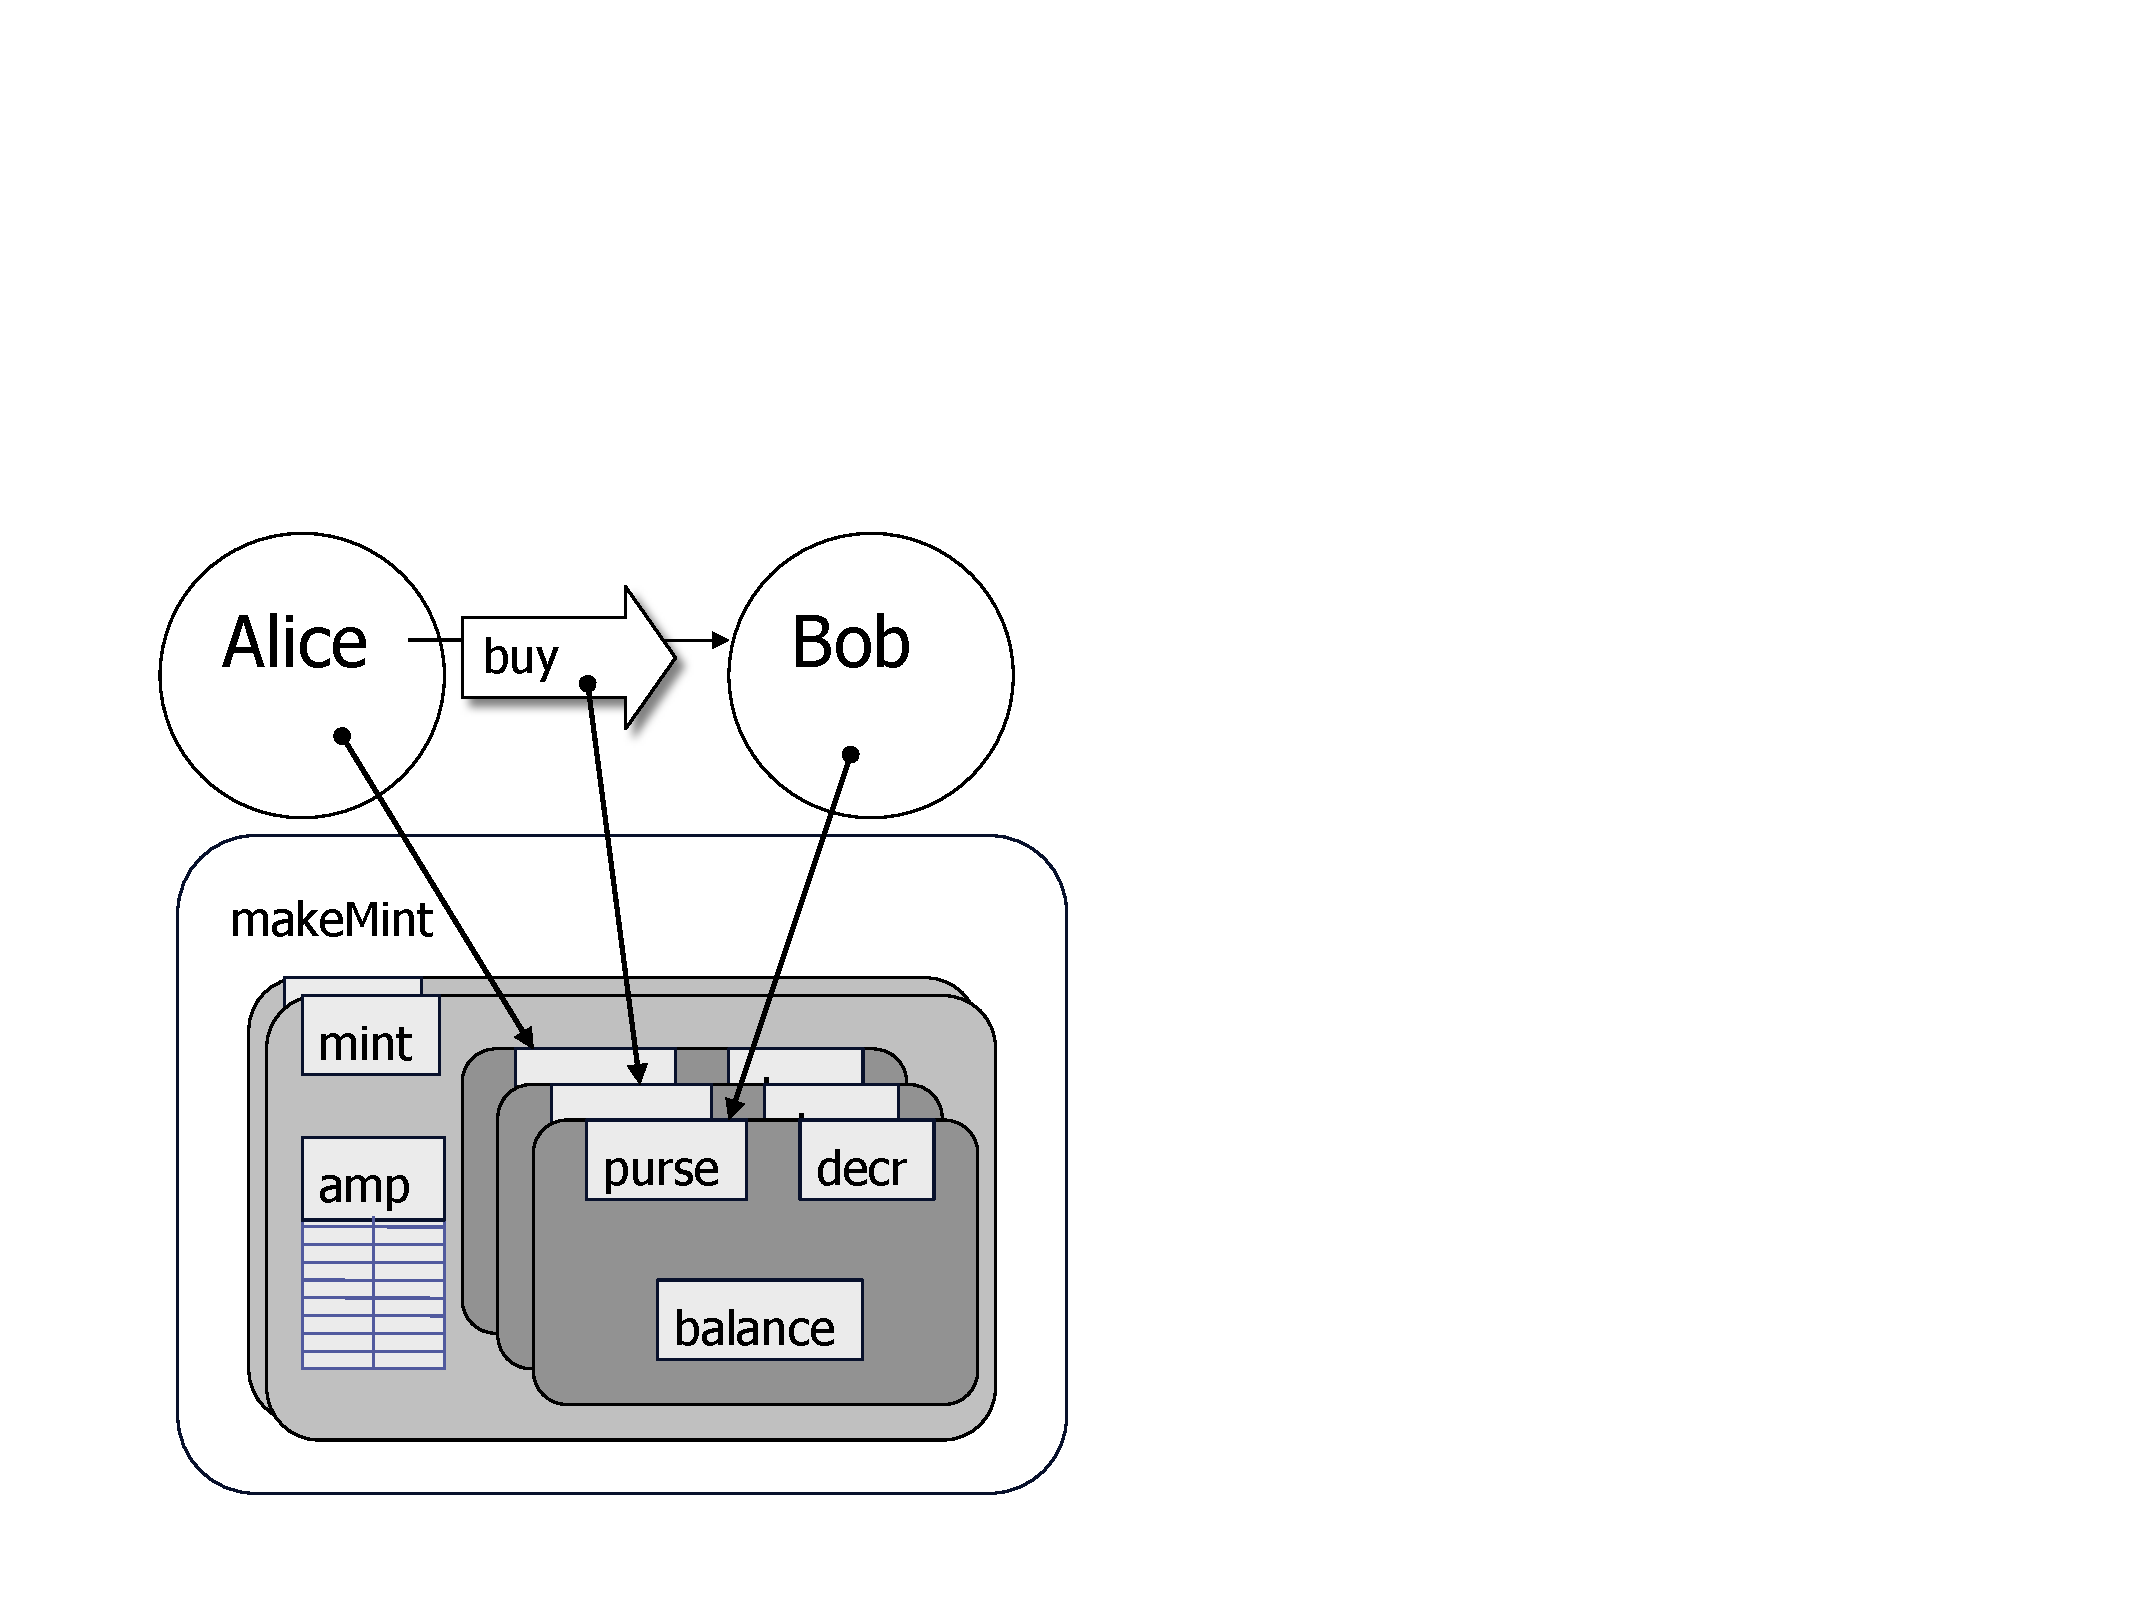
\includegraphics[scale=0.3]{bw-mint.pdf}
\end{minipage}
\caption{The Mint Maker}
\label{makeMint}
\end{figure}

Now that we've seen the elements of Dr. SES, we can proceed to explain how to use it to build electronic rights and smart contracts.

Contracts generally manipulate rights. The participants in a contract each bring to it those rights the contract will manipulate. The logic of the contract together with the decisions of the players determines which derived rights they each walk away with. The simplest example is a direct trade. Since half the rights exchanged in most trades are money, we start with money. 

Figure~\ref{makeMint}  is our implementation of a money-like rights issuer, using only elements of Dr. SES explained above. To explain how it works, it is best to start with how it is used. Say Alice wishes to buy something from Bob for \$10. The three parties involved would be Alice, Bob, and a \$ issuer, which we will informally call a bank. The starting assumptions are that Alice and Bob do not trust each other, the bank does not trust either Alice or Bob, and Alice and Bob trust the bank with their money but with nothing else. In this scenario, Alice is willing to risk her \$10 on the possibility of Bob's non-delivery. But Bob wants to be sure he's been paid before he releases the good in exchange.

What do these relationships mean in terms of a configuration of persistent objects? Say Alice owns (or is) a set of objects on machine A, Bob on machine B, and the bank on machine C. In order for Alice to be able to make a {\tt buy} request of Bob, we assume one of Alice's objects already has a remote reference to one of Bob's objects. Alice's trust of the bank with her money is represented by a remote reference to an object within the bank representing Alice's account at the bank. We refer to such objects as \emph{purses}. The one representing Alice's account is Alice's \emph{main purse}. And likewise for Bob. Where do these initial account purses come from?

For each currency the bank wishes to manage, the bank calls {\tt makeMint()} once to get a {\tt mint} function for making purses holding units of that currency. When Alice opens an account with, say \$100 in cash, the bank calls {\tt mint(100)} on its \$ mint, to make Alice's main purse. The bank then gives Alice a persistent remote reference to this purse object within the bank.

For Alice to pay Bob, she sets up a \emph{payment purse}, deposits \$10 into it from her main purse, and sends it to Bob in a buy request, together with a description of what she wishes to buy.
\begin{verbatim}
  var paymentP = myPurse ! makePurse();
  var ackP = paymentP ! deposit(10, myPurse);
  var goodP = ackP.then(_ => bobP ! buy(desc, paymentP));
\end{verbatim}

On the diagram in Figure~\ref{makeMint}, each {\tt makeMint} call results in a layer with its own {\tt mint}, {\tt amp} pair. Each {\tt mint} call results in a nested layer with its own {\tt purse}, {\tt decr}, {\tt balance} triple. On line 16 of the code that each {\tt purse} to {\tt decr} mapping is also entered into the {\tt amp} table shared by all purses of the same currency. Alice's main purse is on the bottom purse layer. Bob's is on the top layer. Alice's payment purse, being sent to Bob in the buy message, is in the middle layer.

Bob receives this request at the following {\tt buy} method:

\begin{verbatim}
  buy: (desc, paymentP) => {
    // do whatever with desc, look up $10 price
    return (myPurse ! deposit(10, paymentP)).then(
      _ => good,
      // failure handling...
\end{verbatim}

Bob's {\tt buy} method handles a message from untrusted clients such as Alice, and thus it does not know what objects Alice actually provided as the arguments. In particular, Bob has no idea if his {\tt paymentP} parameter actually designates a purse, whether it is a purse at this bank, of this currency, and of adequate funds. Even if he knew all these conditions were true at the moment, since Bob doesn't know whether Alice still retains access to it, Bob wouldn't know the funds would still be there by the time he deposits it. He delegates all these problems to the bank with the {\tt deposit} request above. If the bank's {\tt deposit} method acknowledges a successful deposit, by fulfilling the promise for the result of the deposit, then the success callback of the {\tt then} above gets called, returning the {\tt good}, resolving Alice's pending {\tt goodP} promise.

The interesting work done by {\tt deposit} starts on line 11, where {\tt deposit} looks up the alleged payment purse in the {\tt amp} table. If this is anything other than a purse of the same currency at the same bank, this lookup will instead return undefined, causing the following function call to throw an error. If this lookup succeeds, it finds the {\tt decr} function for decrementing that purse's {\tt balance}, which it calls with the amount to withdraw. If the payment has insufficient funds, {\tt balance - amount} would be negative and {\tt Nat} would throw.

This is the commit point. All the tests that might cause failure have already passed, and no side effects have yet happened. Now we perform all side effects, all of which will happen since no potential locally observable failures remain.
The assignment decrements the payment purse's {\tt balance} by {\tt amount}, and {\tt decr} returns.
Line 12 increments the balance of the purse being deposited into.

This success callback {\tt deposit} method implicitly returns undefined, fulfilling Bob's promise for the result of the {\tt deposit}, triggering Bob to release the good to Alice in exchange.


\section{Towards a Taxonomy of Electronic Rights}

The local unforgeable object reference and the remote unguessable object reference represent one kind of eright---the eright to invoke the public interface of the object it designates. The \emph{mint maker}, building on object references as erights, builds a new kind of eright at a new level of abstraction, one having many of the properties of money. By contrasting these, we can begin to form a taxonomy of erights, and to understand how the layers of abstractions relate to each other. This comparison suggests at least the following four dimensions on which erights may differ.

\begin{center}
\begin{tabular}{ l|l }
  Object reference & Money \\ \hline
  Shared & Exclusive \\
  Specific & Fungible \\
  Opaque & Measurable \\
  Exercisable & Symbolic \\
\end{tabular}\\
\end{center}

When Alice sends the payment purse to Bob, she has \emph{shared} with Bob access to this purse object. If Bob's {\tt deposit} message to his main purse succeeds, Bob obtains \emph{exclusive} access to the money in the purse, denying Alice any further access to that money.

The reference to the payment purse designates a \emph{specific} object, this payment purse as opposed to any other. Whereas the counters in the purses represent only quantities of money (though still specific to a given currency at a given issuer). Bob doesn't care which of these \$s he gets, so long as he gets the amount he expects. The money is \emph{fungible}.

When Bob receives access to the payment purse, he doesn't know what it is except that it is some object that one of his clients chose to send him in this argument position (i.e. the object reference is \emph{opaque}). If his {\tt deposit} method succeeds, he knows exactly what money rights he has received (the money in the purse is \emph{measurable}).

By sending a message to an object, one \emph{exercises} whatever erights to cause effects are provided by that object's public interface. By contrast, money is only valuable because it is valued by others. Money does not have any direct use-value, its value is \emph{symbolic}.

These four dimensions are only a start. Most of the resulting 16 kinds are useful. To have an expressive system of erights, we wish to be able to express many of these easily. But to have a small kernel, we wish to build directly on only the minimal set needed to be able to build the rest easily. Experiments so far, such as the mint maker, indicate that object-references are indeed a good choice of kernel eright.

In this scenario, Alice suffers two vulnerabilities that are less than ideal:
\begin{itemize}
\item Alice must risk her \$10 on the possibility of Bob's non-delivery. We solve this with the next bit of code, the escrow exchange contract, but at the price of exacerbating the next vulnerability.
\item Alice's money is fully vulnerable to misbehavior by the bank. The following escrow exchange scenario protects Alice from Bob's non-delivery, but at the price of vulnerability to \emph{three} third-party services. We return to this issue in section~\ref{futureDirections}.
\end{itemize}



\section{The Escrow Exchange Contract}

\begin{figure}[htbp]
\begin{center}
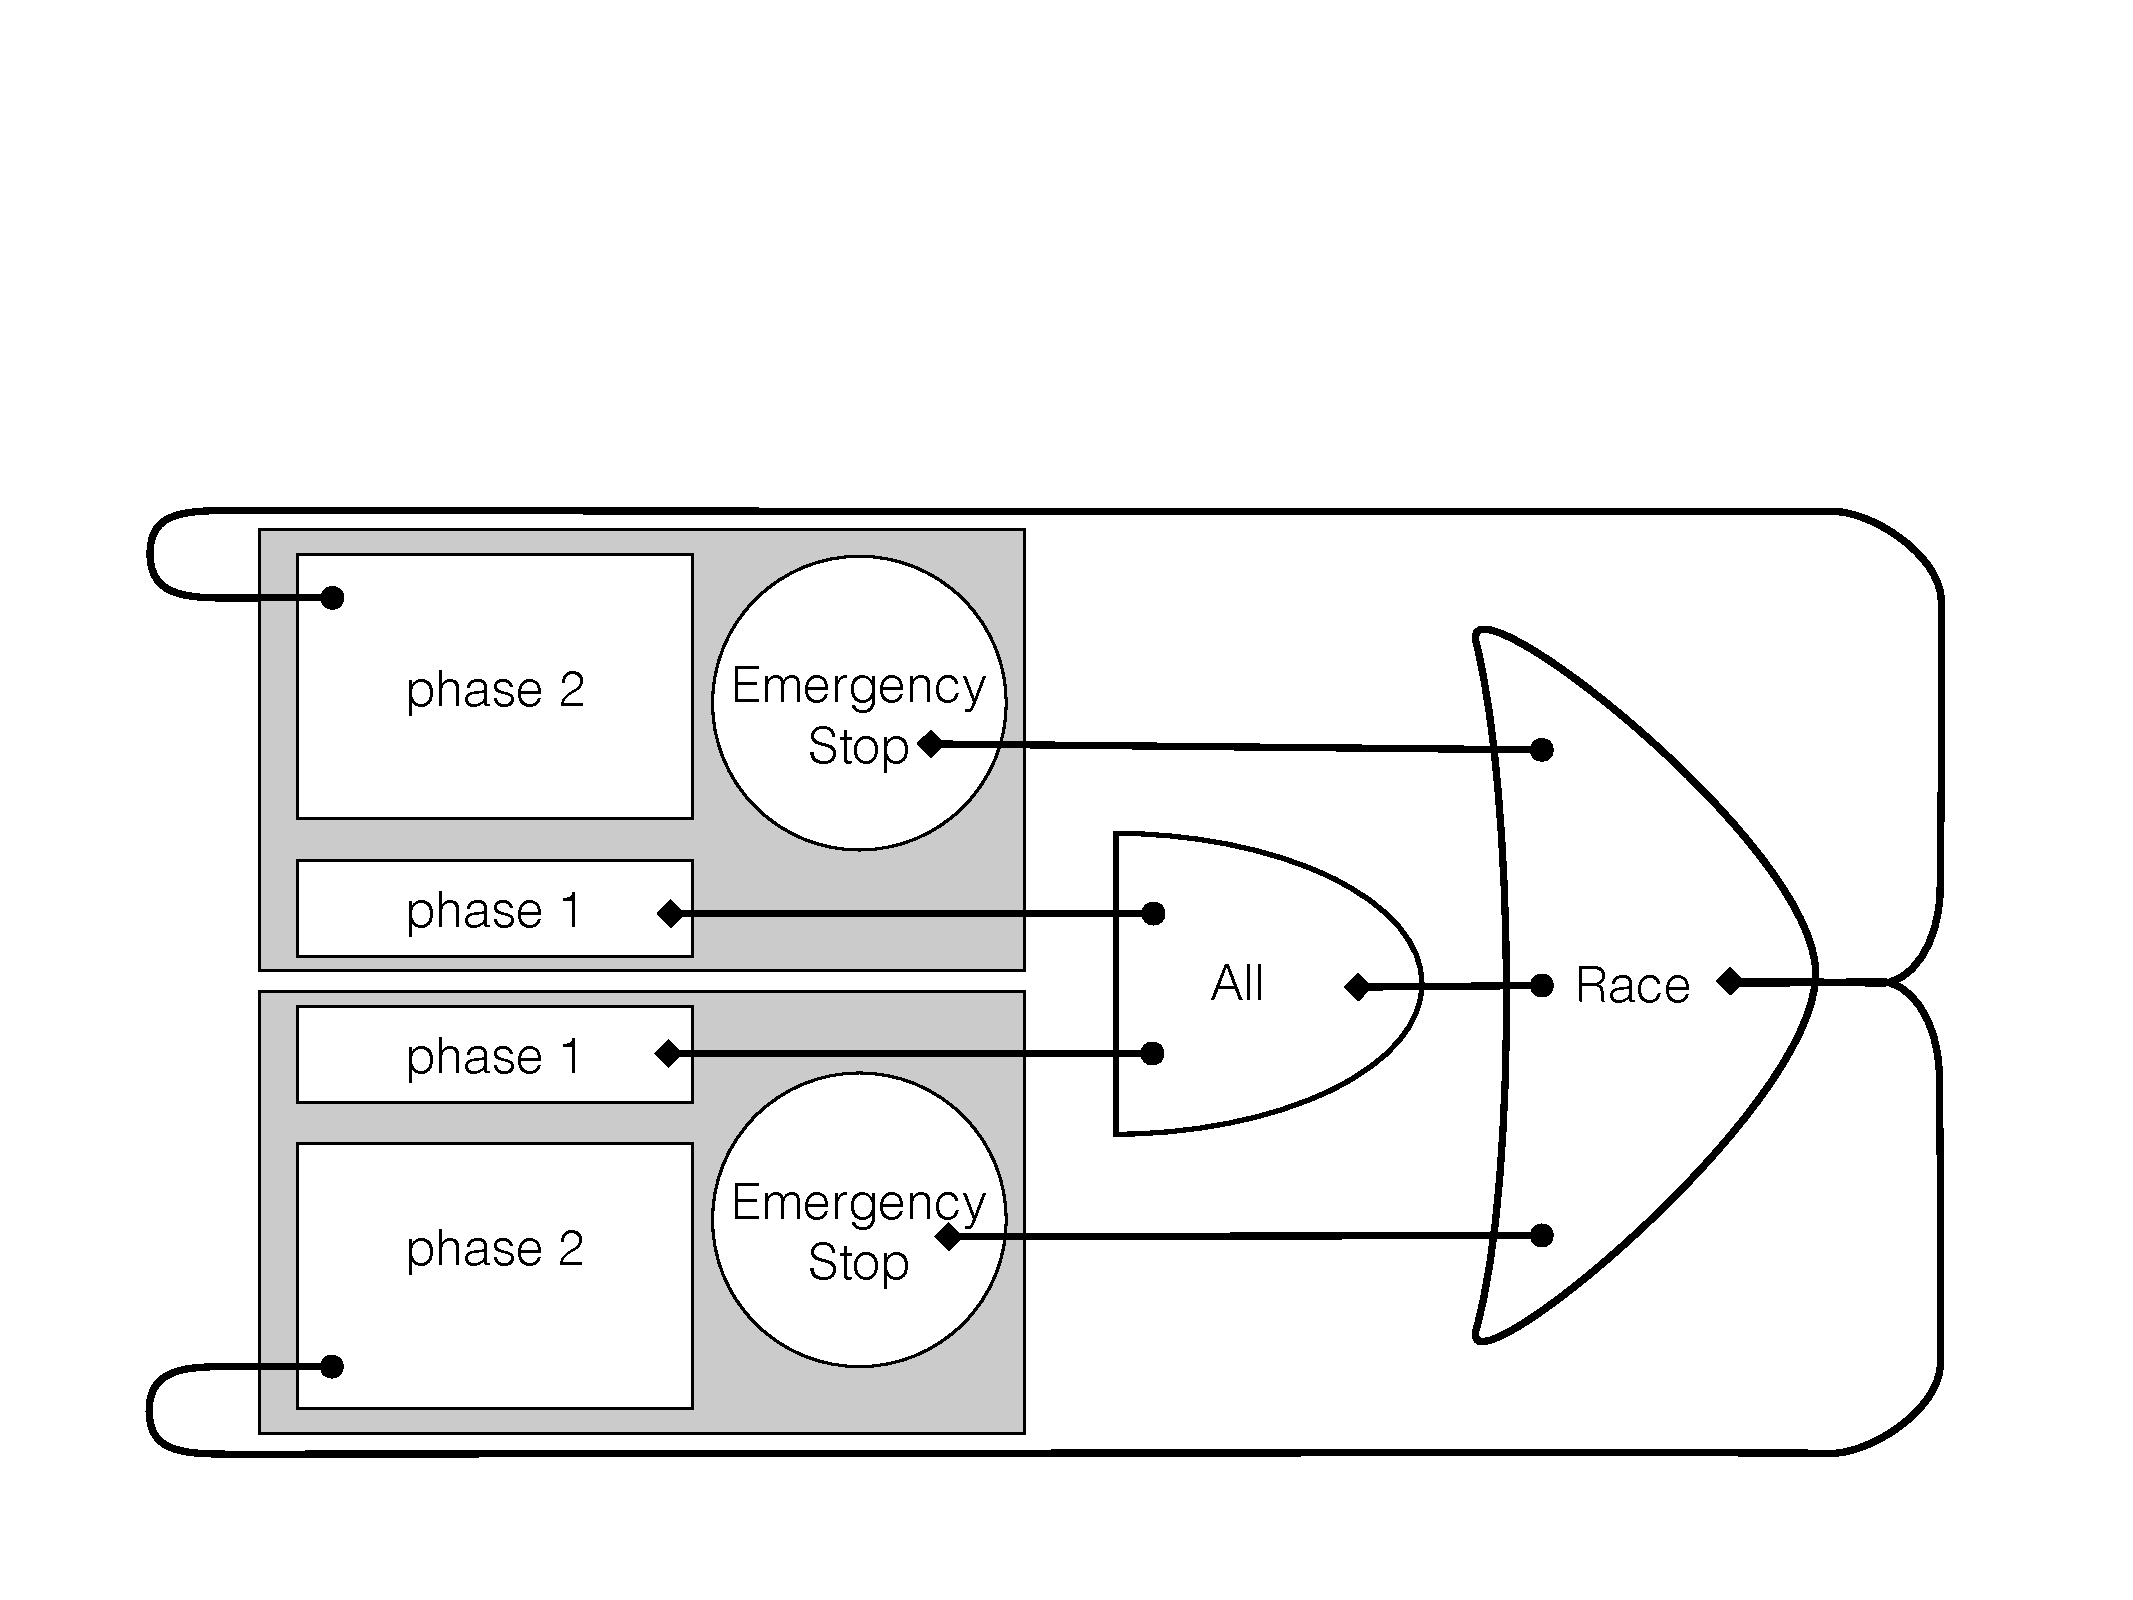
\includegraphics[scale=0.3]{cyclic-circuit.pdf}
\end{center}
\begin{lstlisting}[language=javascript]
var transfer = (decisionP, srcPurseP, dstPurseP, amount) => {
  var makeEscrowPurseP = Q.join(srcPurseP ! makePurse, 
                                   dstPurseP ! makePurse);
  var escrowPurseP = makeEscrowPurseP ! ();

  Q(decisionP).then(                                    // setup phase 2
    _       => { dstPurseP ! deposit(amount, escrowPurseP); },
    reason => { srcPurseP ! deposit(amount, escrowPurseP); });
    
  return escrowPurseP ! deposit(amount, srcPurseP);  // phase 1
};

var failOnly = cancellationP => Q(cancellationP).then(
  cancellation => { throw cancellation; });

var escrowExchange = (a, b) => { // a from Alice, b from Bob
  var decide;
  var decisionP = Q.promise(resolve => { decide = resolve; });

  decide(Q.race([Q.all([
      transfer(decisionP, a.moneySrcP, b.moneyDstP, b.moneyNeeded),
      transfer(decisionP, b.stockSrcP, a.stockDstP, a.stockNeeded)
    ]), 
    failOnly(a.cancellationP), 
    failOnly(b.cancellationP)]));
  return decisionP;
};
\end{lstlisting}
\caption{The Escrow Exchange Contract}
\label{escrowExchange}
\end{figure}

We explain the escrow exchange contract in terms of a scenario among five players, Alice, Bob, a money issuer running the code of Figure~\ref{makeMint}, a stock issuer also running the code of Figure~\ref{makeMint} but with the units representing shares of some particular stock, and an escrow exchange agent running the code of Figure~\ref{escrowExchange}. The diagram at the top of Figure~\ref{makeContractHost} shows the initial relationships, with the escrow exchange agent in the role of contract host.

Alice and Bob again do not trust each other. They wish to trade \$10 of Alice's money for 7 shares of Bob's stock, but in this case, neither is willing to risk their assets on the possibility of the other's non-delivery. They both trust the same money issuer with their money, the same stock issuer with their stock, and the same escrow exchange agent with the rights to be traded. The money issuer, the stock issuer, and the escrow exchange agent each have no prior knowledge or trust in the others. Additionally, none of these trust Alice or Bob. The rest of the scenario as presented below examines only the consequences of Alice or Bob's misbehavior and assumes the other three run the code shown honestly. A full analysis of vulnerabilities should consider all combinations.

Since the situation is now symmetric, we explain the progression of events from Alice's perspective. Alice's prior trust in each issuer is represented as before---Alice holds a persistent reference to her main purse at each issuer. Alice's prior trust in the escrow exchange agent is represented as the ability to provide the first ``{\tt a}'' argument in the call to {\tt escrowExchange} for which Bob is able to provide the second ``{\tt b}'' argument. For this specific interaction, Alice might create this argument as follows:

\begin{verbatim}
  var cancel;
  var a = Q.passByCopy({
    moneySrcP: myMoneyPurse ! makePurse(),
    stockDstP: myStockPurse ! makePurse(),
    stockNeeded: 7,
    cancellationP: Q.promise(r => { cancel = r; });
  });
  moneySrc ! deposit(10, myMoneyPurse);
\end{verbatim}

By a protocol whose details appear below, Alice sends this {\tt a} object to the escrow exchange agent, for it to use as the first argument in a call to {\tt escrowExchange}, which initiates this specific contract between Alice and Bob. The {\tt escrowExchange} function returns a promise for the outcome of the contract, which the escrow exchange agent returns to Alice. 

If this outcome promise becomes fulfilled, the exchange succeeded,  she should expect her {\tt a.moneySrcP} to be drained, and 7 shares of stock to have been deposited into her {\tt a.stockDstP}. If this promise becomes rejected, the exchange failed, and she should expect her {\tt a.moneySrcP} to again hold her \$10. In the meantime, if she gets impatient and would rather not continue waiting, she can call her {\tt cancel} function with her alleged reason for walking away. Once she does so, the exchange will then either succeed or fail promptly.

On lines 13 and 14 of Figure~\ref{escrowExchange} the {\tt escrowExchange} contract makes a {\tt decisionP} promise whose fulfillment or rejection represents its decision about whether the exchange must succeed or fail. It makes this decision by calling {\tt decide} with the outcome of a race between a {\tt Q.all} and two calls to {\tt failOnly}. Until a player cancels the exchange, the {\tt Q.race} can only be won by the {\tt Q.all}, which is where the exchange is proceeding.

The arguments to {\tt Q.all} are the results of two calls to {\tt transfer}. The first call to {\tt transfer} sets up activity whose purpose is to transfer money from Alice to Bob. The second call's purpose is to transfer stock from Bob to Alice. Each call to transfer returns a promise whose fulfillment or rejection indicates whether it has become confident that this one-way transfer of erights would succeed. If both transfers become confident (before any cancellations win the race), then the overall decision is to proceed. If either transfer indicates failure, by rejecting the promise it has returned, then, via {\tt Q.all}, {\tt decisionP} becomes rejected.\footnote{
%
This is the pattern for promise-based two phase commit enhanced with the possibility of cancellation, where the call to {\tt escrowExchange} creates a transaction coordinator, and each of its calls to {\tt transfer} creates a participant.}

We do feed the cancellation promises directly into the race, as Alice could then fulfill the cancellation promise, causing the race to signal a decision to proceed with the exchange, even though Alice's money has not been escrowed, potentially giving Bob's stock to Alice for free. Instead, once the cancellation promise has been either fulfilled or rejected, the promise returned by {\tt failOnly} will only become rejected. Only the {\tt Q.all} can win the race with a success.

Since the two calls to {\tt transfer} are symmetric, we examine only the first. The first phase of the transfer, on line 8 of Figure~\ref{escrowExchange}, attempts to deposit Alice's money into an escrow purse mentioned only within this transfer. If this deposit succeeds, Alice's money has been escrowed, so the money portion of the exchange is now assured. If this deposit fails, then the exchange as a whole should be cancelled. So {\tt transfer} simply returns the promise for the outcome of this first deposit.

The {\tt transfer} function sets up the second phase on lines 5, 6, and 7. If the overall decision is that the exchange should succeed,  the success callback deposits Alice's escrowed money into Bob's account. Otherwise it refunds Alice's money.

Only one mystery remains. How does the escrow agent obtain a fresh escrow purse at this money issuer, in order to be confident that it has obtained exclusive access to the money at stake? Since the escrow exchange agent has no prior knowledge or trust in the money issuer, it cannot become confident that the issuer is honest or even that the money it issues means anything. The question is meaningless. Instead, it only needs to obtain a fresh escrow purse whose veracity is \emph{mutually acceptable} to Alice and Bob.

If it simply asks Alice's purse for a new empty purse ({\tt srcPurseP ! makePurse()}), Alice could return a dishonest purse that acknowledges deposit without transferring anything. Alice would then obtain Bob's stock for free. If it simply asks Bob's purse, then Bob could steal Alice's money during phase 1. Instead, it checks if their {\tt makePurse} methods are the very same function object---have the same object identity--by using {\tt Q.join} on promises for these two methods. This is why, on lines 3 and 7 of Figure~\ref{makeMint}, all purses of the same currency at the same bank share the same function as their {\tt makePurse} method. If the {\tt Q.join} of these two methods fails, the either Alice was dishonest, Bob was dishonest, or they simply didn't have prior agreement on the same currency at the same money issuer.

\section{The Contract Host}
\label{sec:contract_host}

\begin{figure}[htbp]
\begin{minipage}[t]{0.48\linewidth}
\begin{lstlisting}[language=javascript]
var makeContractHost = () => {
  var amp = WeakMap();

  return def({
    setup: contractSrc => {
      contractSrc = ''+contractSrc;
      var tokens = [];
      var argPs = [];
      var resolve;
      var resultP = Q.promise(r => { resolve = r; });
      var contract = confine(contractSrc, {Q: Q});

      var addParam = (i, token) => {
        tokens[i] = token;
        var resolveArg;
        argPs[i] = Q.promise(r => { resolveArg = r; });
        amp.set(token, (allegedSrc, allegedI, arg) => {
          if (contractSrc !== allegedSrc) {
            throw new Error('unexpected contract: '+contractSrc);
          }
          if (i !== allegedI) {
            throw new Error('unexpected side: '+i);
          }
          amp.delete(token);
          resolveArg(arg);
          return resultP;
        });
      };
      for (var i = 0; i < contract.length; i++) {
        addParam(i, def({}));
      }
      resolve(Q.all(argPs).then(args => contract.apply(undefined, args)));
      return tokens;
    },
    play: (tokenP, allegedSrc, allegedI, arg) => Q(tokenP).then(
      token => amp.get(token)(allegedSrc, allegedI, arg))
  });
};
\end{lstlisting}
\end{minipage}
\begin{minipage}[t]{0.48\linewidth}
\vspace{0pt}
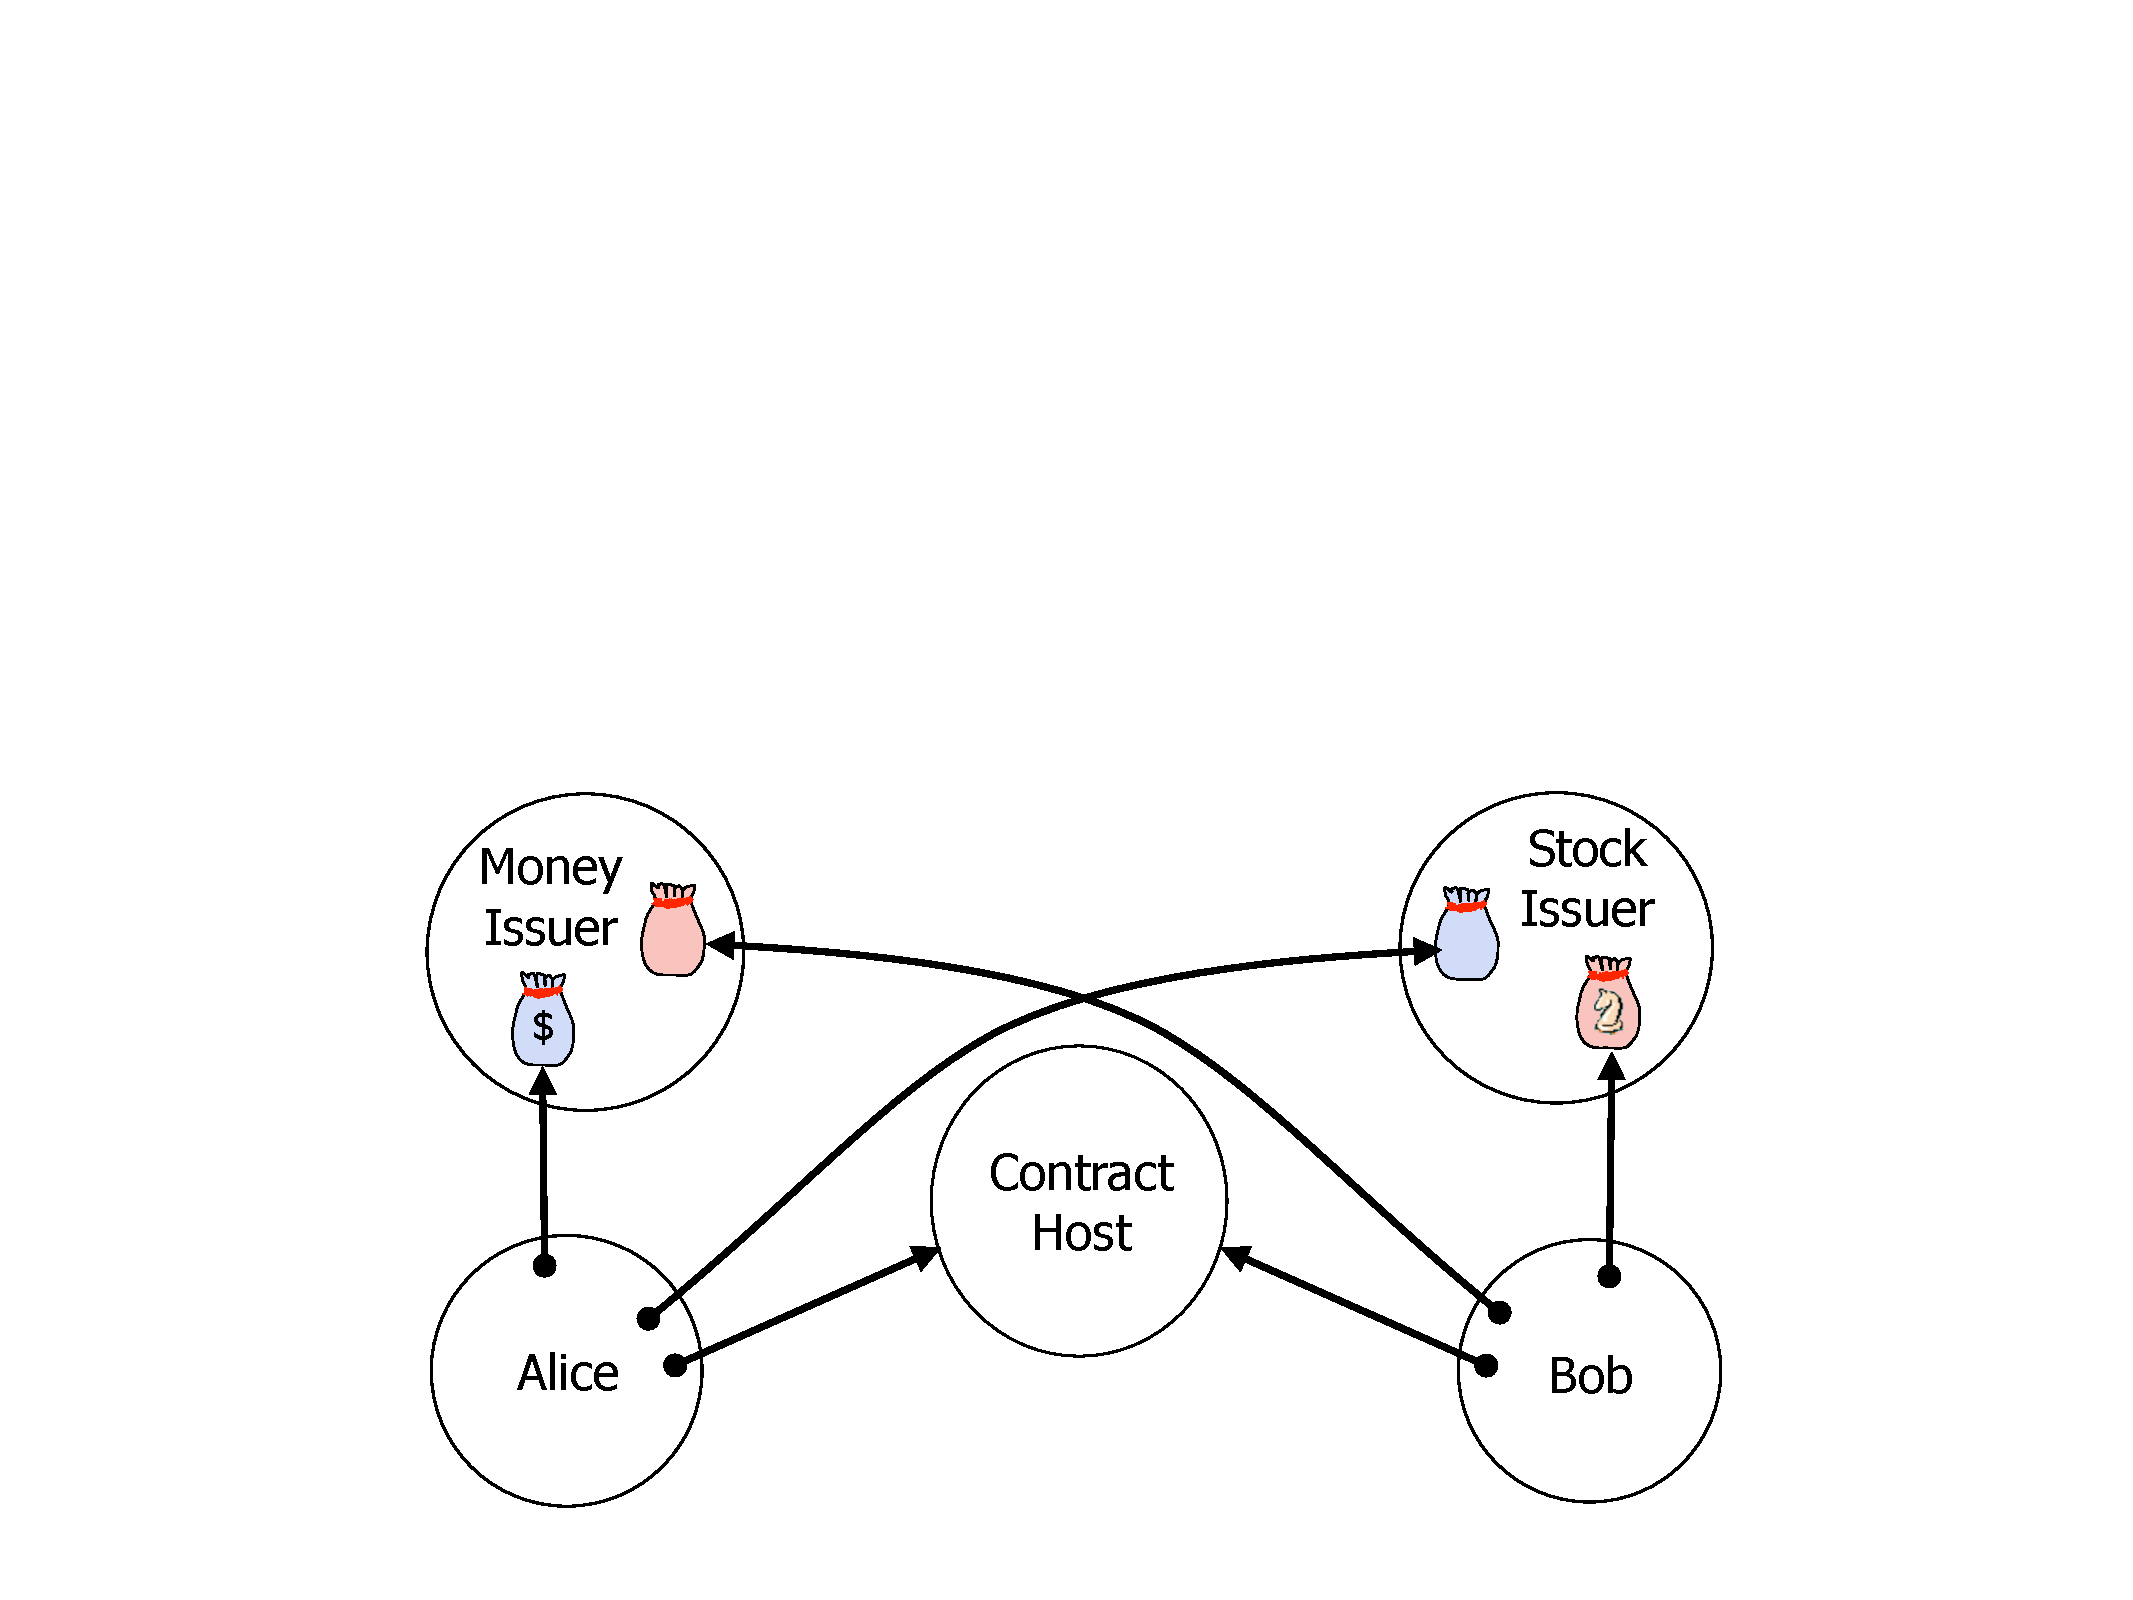
\includegraphics[scale=0.28]{5players.pdf}
\end{minipage}
\caption{The Contract Host}
\label{makeContractHost}
\end{figure}

Once Alice and Bob agree on a contract, how do they arrange for it to be run in a mutually trusted manner?

To engage in the escrow exchange contract, Alice and Bob had to agree on the issuers, which is unsurprising since they need to agree on the nature of rights exchanged by the contract. And they had to agree on an escrow exchange agent to honestly run the escrow exchange contract specifically. For a contract as general as this, perhaps that is not a problem. But if Alice and Bob negotiate a custom contract specialized to their needs, they should not expect to find a mutually trusted third party specializing in running this particular contract. Rather, it should be adequate for them to agree on:

\begin{itemize}
\item The issuers of each of the rights at stake.
\item The source code of the contract.
\item Who is to play which side of the contract.
\item A third party that they mutually trust to run their agreed code, \emph{whatever it is}, honestly.
\end{itemize}

Figure~\ref{makeContractHost} shows the code for a generic contract host. It is able to host any contract formulated, as our escrow exchange contract is, as a function, taking one argument from each player and returning the outcome of the contract as a whole. But setting up a contract is tricky, as it involves a necessary asymmetry among the players. One of the players, say Bob, must initiate a new live contract instance, by sending the contract's code to the contract host. At this point, Bob is the only one who knows both this contract instance and that he'd like to invite Alice to participate in \emph{this} instance. If Bob simply sent to Alice a reference to those objects on the contract host that enables Alice to play, Alice would not know what she's received, since she received it from Bob whom she does not trust. She does trust the contract host, and these objects are on the contract host, but so are the objects corresponding to all the other contracts this host is initiating or running. The connection of Alice to this contract instance must be at Bob's initiation, but Alice's confidence that she's playing the contract she thinks she is much be rooted in her prior trust in the contract host.

Our contract host is an object with two methods, {\tt setup} and {\tt play}. Bob sets up the contract instance by calling {\tt setup} with the source code for the contract function in question, e.g., {\tt escrowExchange}. At line 31, {\tt setup} returns an array of unique unforgeable tokens, one for each argument to the function. Bob's invitation to Alice communicates this token, the source code for the contract he wishes Alice to play, the argument index indicating what side of the contract Alice is to play, and the contract host in question.

If Alice decides she'd like to play this contract, she formulates her argument object as above, and sends it in a {\tt play} request to the contract host along with the token, the alleged contract source code, and the alleged side she is to play. If all of this checks out, and this token has not previously been redeemed, then this token gets used up and Alice's argument is remembered until the arguments for the other players arrive, and Alice receives a promise for the outcome of the contract. Once all arguments are present, the contract function is called and its result is used to resolve the previously returned promise.

By redeeming the token, Alice obtains the exclusive right to play a specific contract whose logic she knows, and whose play she expects to cause external effects. This eright is exclusive, specific, measurable, and exercisable. 

\section{Future Directions}
\label{futureDirections}

\paragraph{Vulnerability to third party services}

Our mint maker is, of course, less than a realistic bank or money system in many ways. Most severe is that Alice's money is \emph{fully vulnerable} to the mint maker's misbehavior, without even the ability to demonstrate such misbehavior to others, to recover losses. Many electronic money systems do better on auditability, but are still ``trusted'' third party services that might misbehave, damaging its clients. A money system, to be useful, must be widely used. A widely used ``trusted'' third party is a central point of failure for a large community.

Better would be to avoid vulnerability to such a central point of failure in the first place. Bitcoin~\cite{nakamoto2008bitcoin} is a virtual issuer, synthesized by cryptographic means among its participants. Rather than rely on a possible malicious third party, Bitcoin arranges a complex system of incentives among the participants, such that the composition of their self-interested behavior within the protocol \emph{should} result in a virtual issuer that is adequately non-subvertable. The game theory has yet to be fully understood, but it is being used at scale, with much value at stake, and has survived many attempted attacks.

One line of research would explore the possible interface between a Bitcoin-like system and Dr. SES. Could a mint-maker-like face be put on Bitcoin, so that it could plug into our escrow exchange agent? But even then, the escrow exchange agent is itself a third party that Alice and Bob are vulnerable to. Can a Bitcoin-like system enable Alice and Bob to synthesize an escrow exchange agent they can both trust without trusting each other? The Bitcoin system already has some "instructions" built into it, specifically intended for supporting smart contracts. But these are currently unused until their implications are better understood. Can the escrow exchange contract be practically compiled into such instructions? In this paper, we have purposely stayed within an extremely small subset of JavaScript. If such an expressive but small language can be compiled into instructions that a Bitcoin-like system can support, could we synthesize a generic contract host, able to host arbitrary contracts written in this language?

\paragraph{Formal verification} 

Previous efforts~\cite{spiessens2007patterns,murray2010analysing} have performed automated verification of the security of several ocap patterns, once expressed in a programming-language independent formalism. Ankur Taly built ENCAP verification system~\cite{taly2011automated} and used it specifically to verify the security of ocap security patterns expressed in concrete SES code. Other researchers have suggested adapting separation logic or ownership types to ocap reasoning. However, the patterns shown here are a bit more complex than those verified to date.

More important, none of these verification systems is in general use, or even understandable by non-specialists. Non-expert programmers reason about the correctness of their programs all the time, but in an informal way best represented as prose arguments. However, as we've seen here, the prose arguments for security can be tricky compared to the those for functionality, mistakes are more likely, and testing is almost useless at identifying holes. In order to enable non-experts to write smart contracts, such tools need to be made understandable and easily usable by those ignorant of the theories on which they are based.





\bibliographystyle{splncs}
% \bibliographystyle{alpha}
\bibliography{common}

\end{document}
